\documentclass[tikz]{standalone}
\usepackage{graphicx} % Required for inserting images
\usepackage{tikz}
\usetikzlibrary{shadows}
\usepackage{xcolor}
\usetikzlibrary{backgrounds}
\usetikzlibrary {shapes.geometric}

\usetikzlibrary {arrows.meta,automata,positioning,fit,calc}

\definecolor{ProcessStepBackground}{HTML}{FFFAF0}
\definecolor{IntermediateStateColour}{HTML}{949698}

\tikzstyle{NetworkLevel} =[draw,trapezium,trapezium stretches body,trapezium left angle=100, trapezium right angle=100]
\tikzstyle{InfinitesimalNode}=[circle,draw=none,inner sep=0pt,minimum size=0pt]
\tikzstyle{ProcessStepNode} =[draw,fill=ProcessStepBackground,rounded corners,text width=2 cm,align=center]
\tikzstyle{IdleState} =[fill=yellow,rounded corners]
\tikzstyle{OutputState} =[fill=red,rounded corners]
\tikzstyle{InputState} =[fill=green,rounded corners]
\tikzstyle{IntermediateState} =[fill=IntermediateStateColour,rounded corners]
\tikzstyle{Source} =[fill=ProcessStepBackground,shape border rotate=90,aspect=0.1,draw]
\tikzstyle{Sink} =[fill=ProcessStepBackground,shape border rotate=90,aspect=0.1,draw]
\tikzstyle{SourceOrSink} =[fill=ProcessStepBackground,cylinder, shape border rotate=90,aspect=0.1,draw,text width=2 cm,align=center]
\tikzset{
diagonal fill/.style 2 args={fill=#2, path picture={
\fill[#1, sharp corners] (path picture bounding box.south west) -|
                         (path picture bounding box.north east) -- cycle;}},
reversed diagonal fill/.style 2 args={fill=#2, path picture={
\fill[#1, sharp corners] (path picture bounding box.north west) |- 
                         (path picture bounding box.south east) -- cycle;}}
}

\tikzstyle{InputAndOutputState} =[diagonal fill={red}{green},rounded corners, drop shadow,draw ]

\begin{document}
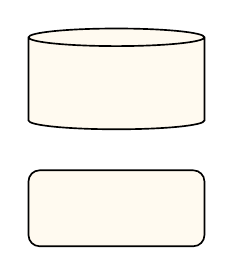
\begin{tikzpicture}[->,auto,node distance=0.5cm,on grid,semithick]
    \node[ProcessStepNode,text opacity=0](Cutting-Machine){Process Step 1-1-1};
    \node[SourceOrSink,above= of Cutting-Machine.north,text opacity=0](Cooled-Toffee-Storage){Storage (Cooled )};

    %     \node[SourceOrSink](Packaged-Toffee-Sink){Sink \\(Packaged Toffee)};
    %     \matrix [column sep=30 mm,row sep=20,draw, rounded corners,nodes={rectangle, anchor=center},NetworkLevel,above= of Packaged-Toffee-Sink.north](6dd744d7-4069-4272-8eaf-f1879d1860a1){
    %         \node[ProcessStepNode](Cutting-Machine){Process Step 1-1-1\\ (Cutting Machine)};     \\
    %         \node[ProcessStepNode](Packaging-Machine){Process Step 1-1-2\\ (Packaging Machine)}; \\
    %     };
    %     \node[SourceOrSink,above= of 6dd744d7-4069-4272-8eaf-f1879d1860a1.north](Cooled-Toffee-Storage){Storage (Cooled Toffee)};
    %     \matrix [column sep=30 mm,row sep=20,draw, rounded corners,nodes={rectangle, anchor=center},NetworkLevel,above= of Cooled-Toffee-Storage.north](b2da0516-bcb6-4dc9-946f-a442e4d4797f){
    %         \node[ProcessStepNode](Toffee-Machine-2){Process Step 2-2-1\\ (Toffee Machine 2)}; &
    %         \node[ProcessStepNode](Toffee-Machine-1){Process Step 2-1-1\\ (Toffee Machine 1)};   \\
    %     };
    %     \node[SourceOrSink,above= of b2da0516-bcb6-4dc9-946f-a442e4d4797f.north](Toffee-Raw-Materials){Source (Toffee Raw Materials)};
    %     \node[,above= of Toffee-Raw-Materials.north](TitleNode){Enterprise};
    %     \draw[dashed] (Cooled-Toffee-Storage) -> (Cutting-Machine);
    %     \draw[] (Cutting-Machine) -> (Packaging-Machine);
    %     \draw[] (Packaging-Machine) -> (Packaged-Toffee-Sink);
    %     \draw[dashed] (Toffee-Raw-Materials) -> (Toffee-Machine-2);
    %     \draw[dashed] (Toffee-Machine-2) -> (Cooled-Toffee-Storage);
    %     \draw[dashed] (Toffee-Raw-Materials) -> (Toffee-Machine-1);
    %     \draw[dashed] (Toffee-Machine-1) -> (Cooled-Toffee-Storage);
\end{tikzpicture}
\end{document}
